\documentclass[UTF8,a4paper]{article}
\usepackage{amsmath, amsfonts, physics, siunitx}
\usepackage{tabularx,tabulary,booktabs}
\usepackage{geometry}
\usepackage{graphicx}
\usepackage{fancyhdr}
\usepackage{float}
\usepackage{enumitem}
\usepackage[colorlinks=true,linkcolor=blue,urlcolor=black,bookmarksopen=true,pdfproducer={xdvipdfmx}]{hyperref}

\geometry{left=2.5cm,right=2.5cm,top=2.54cm,bottom=2.54cm}

\renewcommand{\vec}[1]{\bm{#1}}
% \everymath{\displaystyle}
\lhead{Qiyu Yan}
\rhead{Final Term Report of Computional Computational Physics Course 2020}
\pagestyle{fancy}
\title{Monte Carlo and Molecular Dynamics Simulations of a Lennard–Jones Liquid}
\author{Qiyu Yan\\ \small{2017K8009907053}}


\begin{document}
\maketitle

\tableofcontents
\section{Introduction}
\subsection{Physics Model}
\subsubsection{Cut-off Potential}
In this simulation, I am using Lennard–Jones potential with a cut-off:
\begin{equation}
	U_{i j} \equiv U\left(r_{i j}\right)=\left\{
	\begin{array}{cc}4 \epsilon\left[\left(\frac{\sigma}{r_{i j}}\right)^{12}-\left(\frac{\sigma}{r_{i j}}\right)^{6}\right] & \text { if } r_{i j} \leq r_{c} \\
		0                                                                                                           & \text { if } r_{i j}>r_{c}\end{array}
	\right.
	\label{eqn:l-j}
\end{equation}
By cutting-off Lennard–Jones potential, we can avoid adding infinite periodic particles' contribution to the potential energy calculation.
But there is some price from this cut-off: potential energy will be no longer precise. But the difference should be small that we can estimate the
correction from that.
\subsubsection{Dimensionless Numbers}
All calculations are done with dimensionless numbers, which means by choosing unit as:
\begin{equation}
	\left\{
	\begin{aligned}
		x^{*} & = \frac{x}{\sigma}                                   \\
		v^{*} & = v\frac{t^{*}}{\sigma}                              \\
		t^{*} & = t\left(\frac{\epsilon}{m \sigma^{2}} \right)^{1/2} \\
		E^{*} & = \frac{E}{\epsilon}                                 \\
		T^{*} & = T \frac{k_{\text{B}}}{\epsilon}
	\end{aligned}
	\right.
\end{equation}
By using the left hand variables above, it means that we can emit $\sigma, \, \epsilon, \, k_\text{B}, \, m$ by simply specifying them as ``$1$''
without loss of generality.
\subsubsection{Boundary Conditions}
In this simulation, there is 2 available selections on boundary conditions: \textit{hard boundaries} and \textit{periodic boundary conditions}.
\begin{enumerate}
	\item \textit{Hard Boundaries Conditions}

	      Particles can not exit the box, which means they will be reflected from the walls once trying to leave the box. Different from what in teacher's material
	      I am the particle always reflect in both MC and MD simulation. This makes code reusing easier.
	\item \textit{Periodic Boundary Conditions}

	      Periodic boundary conditions means that there is infinite identical boxes in a true system. One particle leaves from a boundary, another one come in from opposite
	      boundary.
	      \begin{figure}[h]
		      \centering
		      \includegraphics[width=0.3\textwidth]{fig/1024px-Limiteperiodicite.png}
		      \caption{Periodic Boundary Conditions, By I, Grimlock, CC BY-SA 3.0. \href{https://commons.wikimedia.org/wiki/File:Limiteperiodicite.svg}{Link}}
		      \label{fig:Periodic}
	      \end{figure}
	      Of course we will treat the two particle as one. And this also means that when two particle are near different boundaries, that can be ``near'' to each other. So when calculating
	      potential energy and forces, we should always focus on the nearest choose in all possible periodic positions.

	      This can be done with trick, give 1-D situation for example: two particle's position difference can be expressed by a scalar $\Delta x = x_1 - x_2$, in a periodic boundary system with
	      period is $L$, that the best choice for their position difference in all available periodic can be chosen as:
	      \begin{equation}
		      \Delta x' = \left(\Delta x + \frac{L}{2}\right)\bmod L - \frac{L}{2}
		      \label{eqn:periodic}
	      \end{equation}
	      Expanding this formula to 2-D or n-D situation is trivial, just by applying \eqref{eqn:periodic} to all dimension, and when all dimension has a smallest distance, the total distance will
	      be minimized.

	      And for a periodic system with a period $L > r_c$, see \eqref{eqn:l-j}, there cannot be more than one choice that makes $r < r_c$, so we should focus only on the minimized one. So
	      \textit{calculate the interaction energies for each particle by summing up the pair interactions with all the neighbors within the chosen cut-off distance} is reduced to calculate the minimized periodic
	      distance for each pair particle, this can definitely speed up the calculation.
\end{enumerate}
\subsection{Coding}
This time all coding work is done with Python, and NumPy makes my program much faster than using loops, maximize the usage of ufunc and vectorized calculation. And do avoid any possible copies is important.
And since I am using class in Python to make coding simpler.

\subsubsection{Code Structure}
My code contains those modules:
\begin{enumerate}
	\item configuration

	      Define general particle system behavior and methods, such as placing particle, calculating potential energy, proceeding periodic boundaries in class \textbf{physics\underline{~~}system}, the class will be base class for
	      \textbf{physical\underline{~~}system\underline{~~}monte\underline{~~}carlo} and \textbf{molecular\underline{~~}dynamics\underline{~~}system}.
	\item lennard\underline{~~}jones\underline{~~}potential

	      Functions for Lennard–Jones potential related calculating, including calculating total potential energy, potential energy related to one particle, force on each particle. All codes are vectorized by NumPy to make calculating
	      faster.
	\item molecular\underline{~~}dynamics

	      \begin{itemize}
		      \item Class \textbf{molecular\underline{~~}dynamics\underline{~~}system}, derived from \textbf{physics\underline{~~}system}, adds functions to assign velocities by certain temperature, doing adiabatic or thermostatic iteration
		            on the system. And added class methods to get total energy, total kinetic energy, which will be useful when doing checks.
		      \item Class \textbf{molecular\underline{~~}dynamics}, a wrapper to initialize \textbf{molecular\underline{~~}dynamics\underline{~~}system}, do iteration and save interested information from \textbf{molecular\underline{~~}dynamics\underline{~~}system}
	      \end{itemize}
	\item monte\underline{~~}carlo

	      \begin{itemize}
		      \item Class \textbf{monte\underline{~~}carlo\underline{~~}system}, similar to \textbf{molecular\underline{~~}dynamics\underline{~~}system}, this is derived from \textbf{physics\underline{~~}system}, by adding functions to do Metropolis
		            iteration.
		      \item Class \textbf{monte\underline{~~}carlo} a wrapper to initialize \textbf{monte\underline{~~}carlo\underline{~~}system} and save useful information for later usage.
	      \end{itemize}
	\item test\underline{~~}cases

	      Since most code is contained into classes, and testing class by \textbf{doctest} is not a easy work, so I switched to \textbf{PyTest}. PyTest is a testing framework whose test cases itself is a piece of Python code. Using Python code to test python is
	      easier than using doctest's string match.
\end{enumerate}
But the testing cases didn't cover anything, I didn't come up a way to test molecular dynamics code automatically, so I did that manually, by checking during several adiabatic iterations, if total energy conserves and if center of mass velocity remains to be zero. During
those checking, I found some interesting problem arose, which will be talked about later.

\section{Equilibration}
Setting fixed temperature $\rho$ and density $T$, run Monte Carlo simulations and molecular dynamics simulations to gain potential energy per step, and calculate
$\expval{U} = \frac{1}{N}\sum_{T=1}^N U(T)$
\subsection{$T =0.728,\, \rho = 0.8442$}

First, by a long time simulation on periodic Monte Carlo with random initialized position, I can draw a scatter plot of the ``final state''. As in Figure \ref{fig:scatter},
\begin{figure}[h]
	\centering
	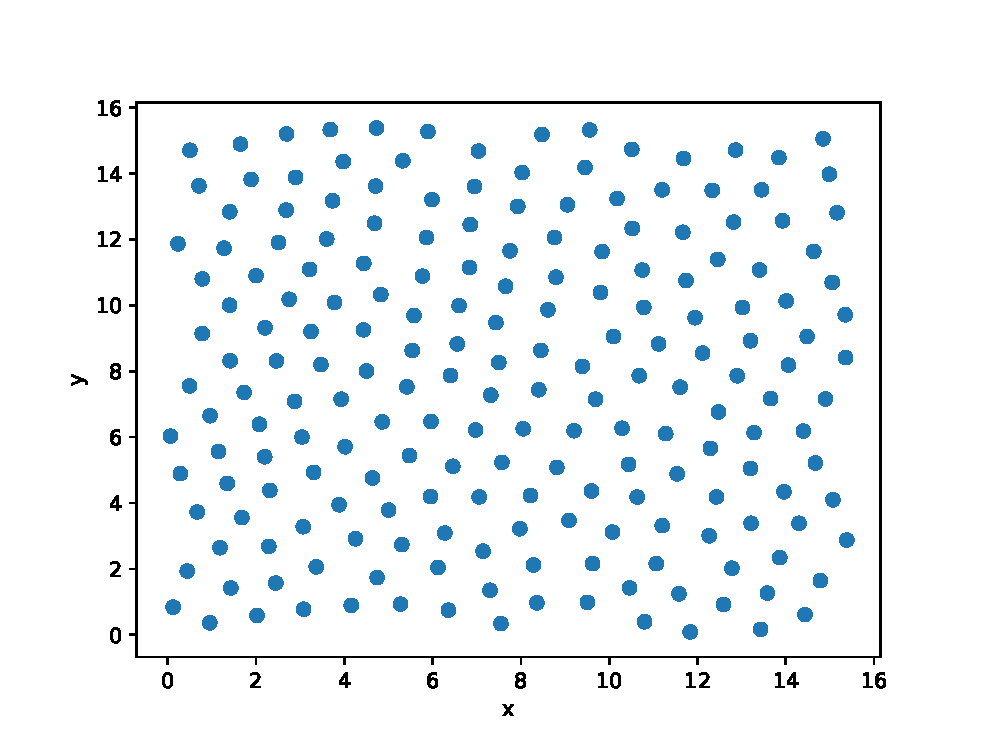
\includegraphics[width=0.4\textwidth]{fig/rand_scatter_70000_steps_200_particles_0.8442_rho_0.728_tempure_.eps}
	\caption{Monte Carlo with random initialized position, $T_1 =0.728,\, \rho_1 = 0.8442$, 70000 steps with 200 particles}
	\label{fig:scatter}
\end{figure}

Here, we can see some hexagonal like clusters in the figure, so, in the following code, I will use hexagonal lattice as non-random initialization.

When doing molecular dynamics with random initializing, there is a problem that total energy (potential+kinetic) always change, after looking into the problem, it seems that the force on
particles can be extremely high ($1\times 10^{8}$) for first step, this makes the simulation broken. The problem is from the high potential energy of random placement. So, before iteration by
molecular dynamics methods, I have performed 1000 Monte Carlo iterations to lower the potential energy.
\subsubsection{Random Placement, Periodic Boundaries}
First choose random placement as initialize configuration, and we can get that:
\begin{figure}[H]
	\centering
	\begin{minipage}[t]{0.45\textwidth}
		\centering
		\includegraphics[height=0.2\textheight]{fig/plot_norand_30000_steps_100_particles_0.8442_rho_0.728_tempure_.eps}
		\caption{Random placement, Monte Carlo simulation, at 30000 steps, with 100 particles}
	\end{minipage}\hspace{0.5cm}
	\begin{minipage}[t]{0.45\textwidth}
		\centering
		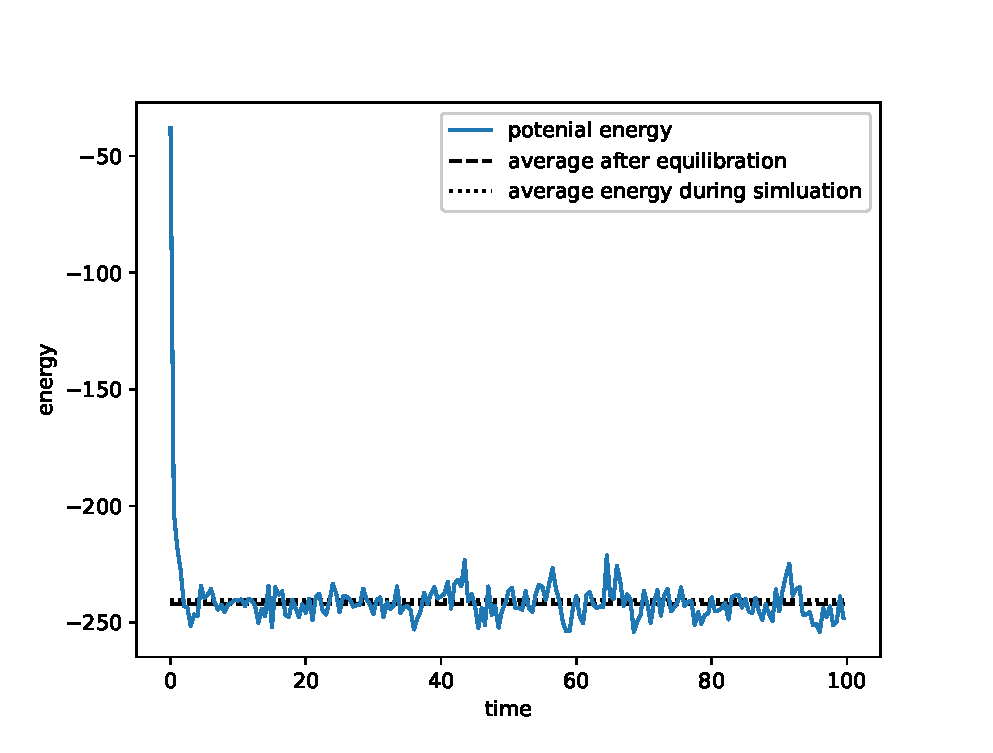
\includegraphics[height=0.2\textheight]{fig/md_plot_20000_steps_100_particles_0.8442_rho_0.728_tempure_.eps}
		\caption{Random placement, molecular dynamics simulation, at 20000 steps, with 100 particles, time step is $0.05$}
	\end{minipage}
\end{figure}
And the calculated total potential energy and its fluctuation are in Table \ref{tab:rand1}:
\begin{table}[H]
	\centering
	\caption{Random placement, periodic boundaries}
	\begin{tabular}{rcc}
		\toprule
		\toprule
		                       & Monte Carlo & molecular dynamics \\ \midrule
		total potential energy & $-230.15$   & $-242.64$          \\
		square fluctuation     & $34.1$      & $41.4$             \\
		fluctuation            & $5.83$      & $6.43$             \\
		\bottomrule
	\end{tabular}%
	\label{tab:rand1}%
\end{table}%  
Fluctuation $\delta U$ in table \ref{tab:rand1} is defined as:
\begin{equation}
	\delta U^{2}=\expval{U^2} - \expval{U}^2	\label{eq:flu}
\end{equation}

But the fluctuation and total potential energy can change between runs, the number is a random chosen one. Change in fluctuation may come from size,
we have learnt that total energy fluctuation is proportional to its temperature and the fluctuation of fluctuation is proportional to its size.
This can be verified by changing it size and calculate $\frac{\delta U}{N}$,
it is all near $0.05$ for this temperature/density selection.

\subsubsection{Hexagonal Lattice, Periodic Boundaries}
I set initial configuration for the particles with hexagonal lattice with $r = 1.1$, the number is near the lowest energy for the lattice Structure.
\begin{figure}[H]
	\centering
	\begin{minipage}[t]{0.45\textwidth}
		\centering
		\includegraphics[height=0.2\textheight]{fig/plot_40000_steps_100_particles_0.8442_rho_0.728_tempure_1.eps}
		\caption{Hexagonal placement, periodic boundaries, Monte Carlo simulation, at 40000 steps, with 100 particles}
	\end{minipage}\hspace{0.5cm}
	\begin{minipage}[t]{0.45\textwidth}
		\centering
		\includegraphics[height=0.2\textheight]{fig/md_plot_norand__10000_steps_100_particles_0.8442_rho_0.728_tempure_.eps}
		\caption{Hexagonal placement, periodic boundaries, molecular dynamics simulation, at 20000 steps, with 100 particles, time step is $0.05$}
	\end{minipage}
\end{figure}
\begin{table}[H]
	\centering
	\caption{Hexagonal placement, periodic boundaries}
	\begin{tabular}{rcc}
		\toprule
		\toprule
		                       & Monte Carlo & molecular dynamics \\ \midrule
		total potential energy & $-242.97$   & $-241.15$          \\
		square fluctuation     & $31.9$      & $42.2$             \\
		fluctuation            & $5.65$      & $6.53$             \\
		\bottomrule
	\end{tabular}%
	\label{tab:hex1}%
\end{table}%  
As in Table \ref{tab:hex1}, total potential energy results from the two simulation is very close, while there is still some difference
in the fluctuation.
\subsubsection{Random Placement, Hard Boundaries}
\begin{figure}[H]
	\centering
	\begin{minipage}[t]{0.45\textwidth}
		\centering
		\includegraphics[height=0.2\textheight]{fig/plot_hb_80000_steps_100_particles_0.8442_rho_0.728_tempure_1.eps}
		\caption{Random placement, hard boundaries, Monte Carlo simulation, at 80000 steps, with 100 particles}
	\end{minipage}\hspace{0.5cm}
	\begin{minipage}[t]{0.45\textwidth}
		\centering
		\includegraphics[height=0.2\textheight]{fig/md_plot_rand_hard_10000_steps_100_particles_0.8442_rho_0.728_tempure_.eps}
		\caption{Random placement, hard boundaries, molecular dynamics simulation, at 10000 steps, with 100 particles, time step is $0.05$}
	\end{minipage}
\end{figure}
\begin{table}[H]
	\centering
	\caption{Hexagonal placement, periodic boundaries}
	\begin{tabular}{rcc}
		\toprule
		\toprule
		                       & Monte Carlo & molecular dynamics \\ \midrule
		total potential energy & $-192.47$   & $-191.12$          \\
		square fluctuation     & $24.7$      & $25.6$             \\
		fluctuation            & $4.97$      & $5.05$             \\
		\bottomrule
	\end{tabular}%
	\label{tab:rand_hard1}%
\end{table}%  
As in Table \ref{tab:rand_hard1}, compared to Table \ref{tab:rand1}, we can see some difference in \textit{total potential energy}, and a slightly smaller \textit{fluctuation},
this difference is from the size effect from the hard boundaries.

\subsubsection{Hexagonal Lattice, Hard Boundaries}
\begin{figure}[H]
	\centering
	\begin{minipage}[t]{0.45\textwidth}
		\centering
		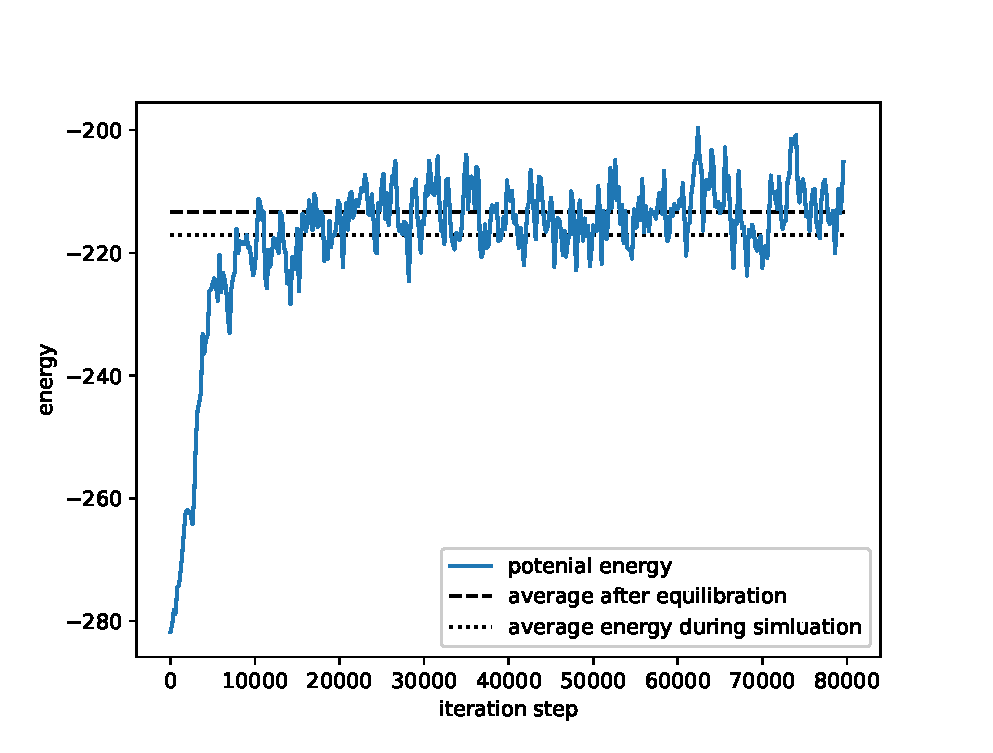
\includegraphics[height=0.2\textheight]{fig/plot_hb_norand_80000_steps_100_particles_0.8442_rho_0.728_tempure_1.eps}
		\caption{Hexagonal placement, hard boundaries, Monte Carlo simulation, at 80000 steps, with 100 particles}
	\end{minipage}\hspace{0.5cm}
	\begin{minipage}[t]{0.45\textwidth}
		\centering
		\includegraphics[height=0.2\textheight]{fig/md_plot_norand_hard_10000_steps_100_particles_0.8442_rho_0.728_tempure_.eps}
		\caption{Hexagonal placement, hard boundaries, molecular dynamics simulation, at 10000 steps, with 100 particles, time step is $0.05$}
	\end{minipage}
\end{figure}
\begin{table}[H]
	\centering
	\caption{Hexagonal placement, periodic boundaries}
	\begin{tabular}{rcc}
		\toprule
		\toprule
		                       & Monte Carlo & molecular dynamics \\ \midrule
		total potential energy & $-213.32$   & $-193.21$          \\
		square fluctuation     & $21.7$      & $27.40$            \\
		fluctuation            & $4.66$      & $5.23$             \\
		\bottomrule
	\end{tabular}%
	\label{tab:hex2}%
\end{table}%  
There is a significant difference in the \textit{total potential energy} between two simulation method here, this may suggest that reflecting on the wall can not represent ``the truth''.

\subsubsection{Tail Correction}
The calculation of tail correction, as listed in the book (3.2.2), can be written as:
\begin{equation}
	U^{\text{tail}} = \frac{N \rho}{2} \int_{r_{c}}^{\infty} \operatorname{dr} u(r) 2 \pi r.
\end{equation}
This is trivial for periodic boundaries and $L>r_c$. So, by doing this integration with Mathematica, it gives:
\begin{equation}
	\begin{aligned}
		U^{\text{tail}} & = \frac{N \rho}{2} \int_{r_{c}}^{\infty} \operatorname{dr} u(r) 2 \pi r              \\
		                & = \frac{N \rho \epsilon \pi \sigma^6\left(-5 r_c^6 + 2 \sigma^6\right)}{5 r_c^{10}}.
	\end{aligned}
	\label{eq:tail}
\end{equation}
Let $r_c = 2.5, \, \sigma = \epsilon = 1, \,\rho = 0.8442, \,N = 100$, it gives:
\begin{equation*}
	U^{\text{tail}}_{\text{periodic}} = -6.778\,.
\end{equation*}
For hard boundaries, particle distance has a upper limit, in this case, the upper limit is near half its system length, so we should not take count of those part.
\begin{equation*}
	U^{\text{tail}}_{\text{hard}} \approx -6.778 + 0.424 = -6.353 \,.
\end{equation*}

\subsection{$T =1.0,\, \rho = 0.1$}
\subsubsection{Random Placement, Periodic Boundaries}
First choose random placement as initialize configuration, and we can get that:
\begin{figure}[H]
	\centering
	\begin{minipage}[t]{0.45\textwidth}
		\centering
		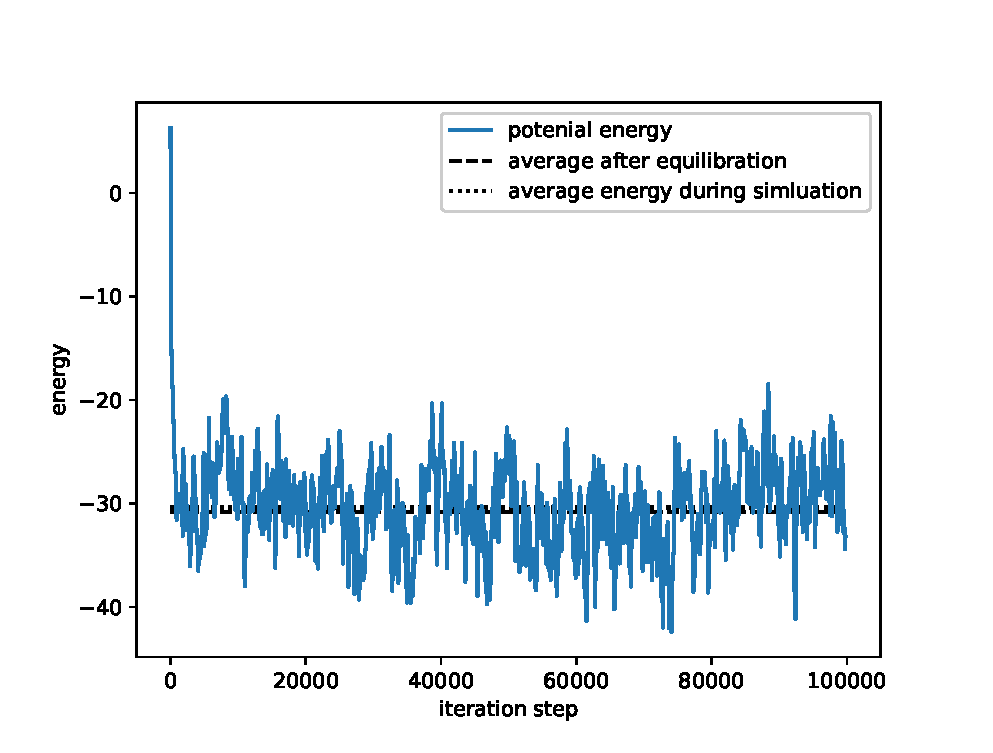
\includegraphics[height=0.2\textheight]{fig/exp2_rand_peri_mc.eps}
		\caption{Random placement, Monte Carlo simulation, at 100000 steps, with 100 particles}
	\end{minipage}\hspace{0.5cm}
	\begin{minipage}[t]{0.45\textwidth}
		\centering
		\includegraphics[height=0.2\textheight]{fig/exp2_rand_peri_md.eps}
		\caption{Random placement, molecular dynamics simulation, at 20000 steps, with 100 particles, time step is $0.05$}
	\end{minipage}
\end{figure}
And the calculated total potential energy and its fluctuation are in Table \ref{tab:rand_p}:
\begin{table}[H]
	\centering
	\caption{Random placement, periodic boundaries}
	\begin{tabular}{rcc}
		\toprule
		\toprule
		                       & Monte Carlo & molecular dynamics \\ \midrule
		total potential energy & $-30.83$    & $-24.51$           \\
		square fluctuation     & $16.9$      & $15.8$             \\
		fluctuation            & $4.12$      & $3.98$             \\
		\bottomrule
	\end{tabular}%
	\label{tab:rand_p}%
\end{table}%  

\subsubsection{Hexagonal Lattice, Periodic Boundaries}
\begin{figure}[H]
	\centering
	\begin{minipage}[t]{0.45\textwidth}
		\centering
		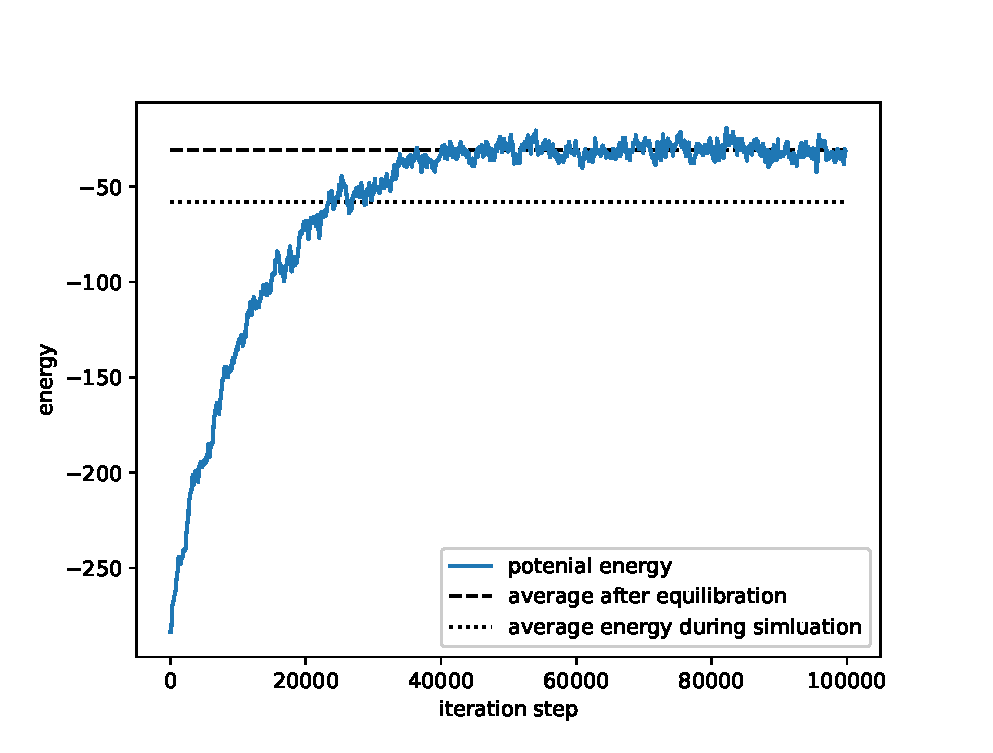
\includegraphics[height=0.2\textheight]{fig/exp2_hex_peri_mc.eps}
		\caption{Hexagonal placement, periodic boundaries, Monte Carlo simulation, at 100000 steps, with 100 particles}
	\end{minipage}\hspace{0.5cm}
	\begin{minipage}[t]{0.45\textwidth}
		\centering
		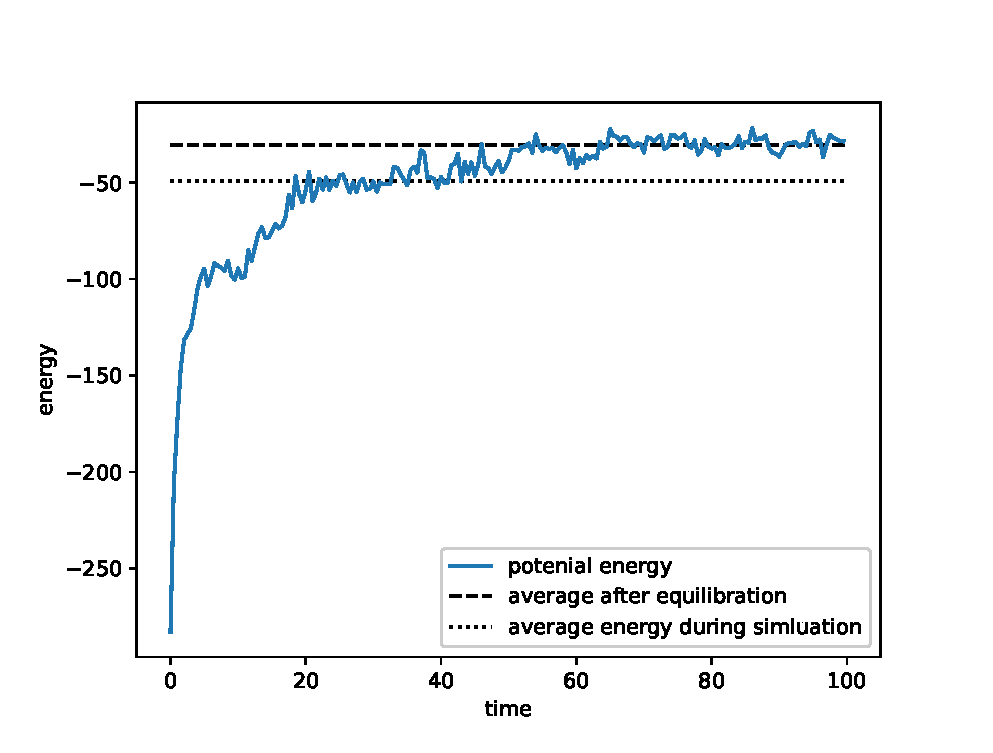
\includegraphics[height=0.2\textheight]{fig/exp2_hex_peri_md.eps}
		\caption{Hexagonal placement, periodic boundaries, molecular dynamics simulation, at 20000 steps, with 100 particles, time step is $0.05$}
	\end{minipage}
\end{figure}
\begin{table}[H]
	\centering
	\caption{Hexagonal placement, periodic boundaries}
	\begin{tabular}{rcc}
		\toprule
		\toprule
		                       & Monte Carlo & molecular dynamics \\ \midrule
		total potential energy & $-30.79$    & $-30.61$           \\
		square fluctuation     & $15.0$      & $16.2$             \\
		fluctuation            & $3.86$      & $4.02$             \\
		\bottomrule
	\end{tabular}%
	\label{tab:hex_md_1}%
\end{table}%  

\subsubsection{Random Placement, Hard Boundaries}
\begin{figure}[H]
	\centering
	\begin{minipage}[t]{0.45\textwidth}
		\centering
		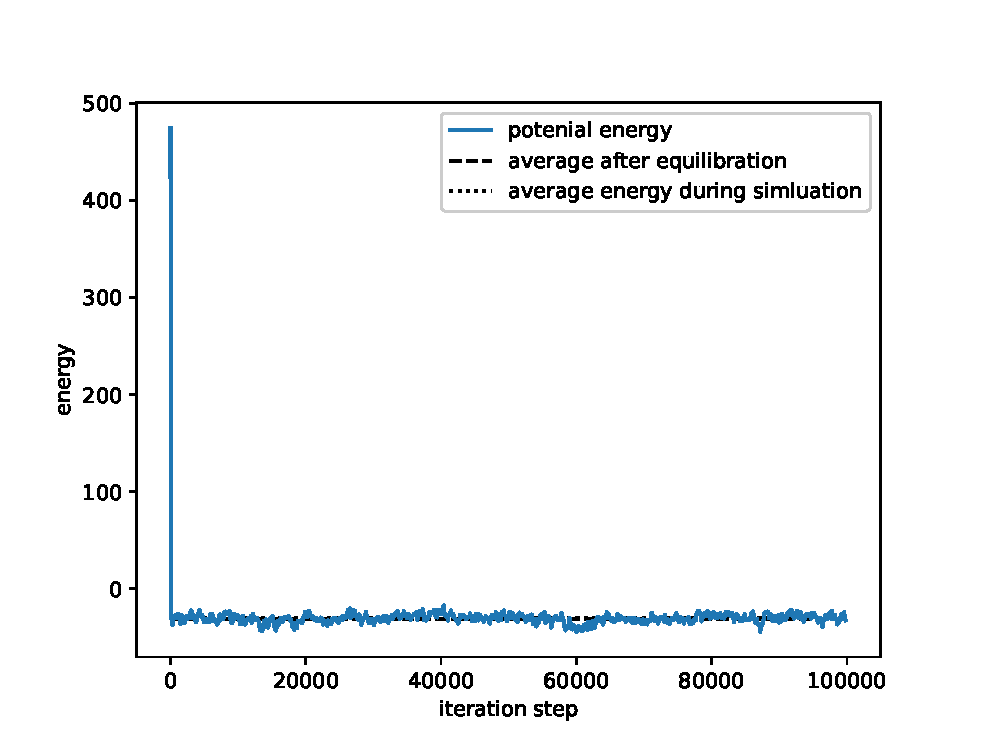
\includegraphics[height=0.2\textheight]{fig/exp2_rand_hard_mc.eps}
		\caption{Random placement, hard boundaries, Monte Carlo simulation, at 100000 steps, with 100 particles}
	\end{minipage}\hspace{0.5cm}
	\begin{minipage}[t]{0.45\textwidth}
		\centering
		\includegraphics[height=0.2\textheight]{fig/exp2_rand_hard_md.eps}
		\caption{Random placement, hard boundaries, molecular dynamics simulation, at 20000 steps, with 100 particles, time step is $0.05$}
	\end{minipage}
\end{figure}
\begin{table}[H]
	\centering
	\caption{Hexagonal placement, periodic boundaries}
	\begin{tabular}{rcc}
		\toprule
		\toprule
		                       & Monte Carlo & molecular dynamics \\ \midrule
		total potential energy & $-31.08$    & $-21.89$           \\
		square fluctuation     & $19.3$      & $17.4$             \\
		fluctuation            & $4.38$      & $4.17$             \\
		\bottomrule
	\end{tabular}%
	\label{tab:rand_hard_2}%
\end{table}%  

\subsubsection{Hexagonal Lattice, Hard Boundaries}
\begin{figure}[H]
	\centering
	\begin{minipage}[t]{0.45\textwidth}
		\centering
		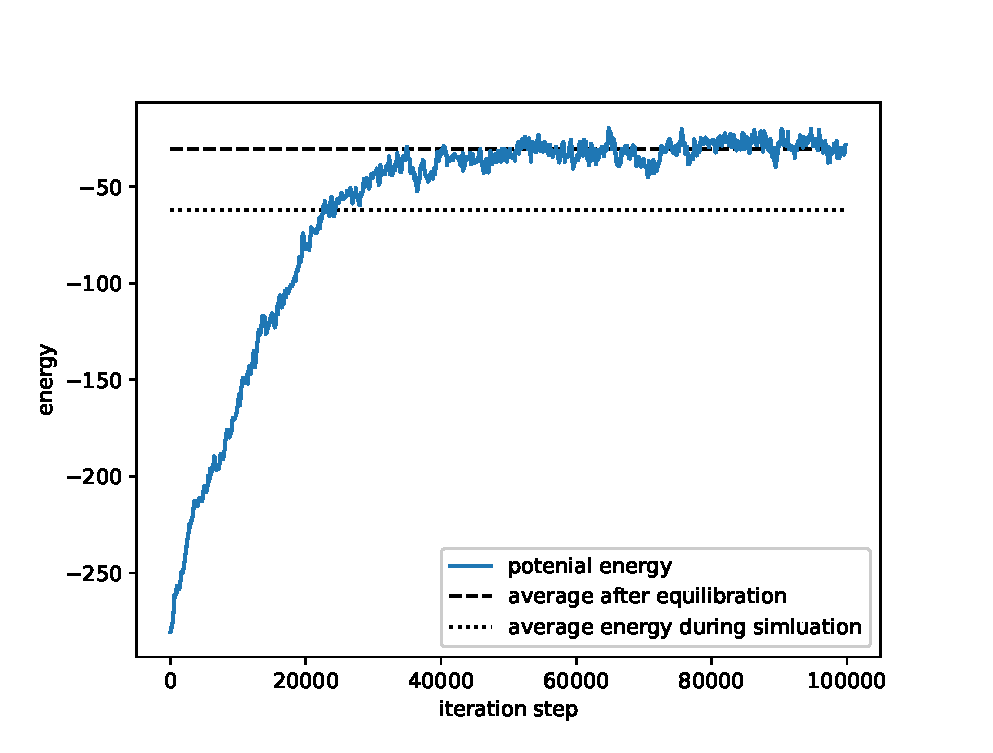
\includegraphics[height=0.2\textheight]{fig/exp2_hex_hard_mc.eps}
		\caption{Hexagonal placement, hard boundaries, Monte Carlo simulation, at 80000 steps, with 100 particles}
	\end{minipage}\hspace{0.5cm}
	\begin{minipage}[t]{0.45\textwidth}
		\centering
		\includegraphics[height=0.2\textheight]{fig/md_plot_norand_hard_10000_steps_100_particles_0.8442_rho_0.728_tempure_.eps}
		\caption{Hexagonal placement, hard boundaries, molecular dynamics simulation, at 10000 steps, with 100 particles, time step is $0.05$}
	\end{minipage}
\end{figure}
\begin{table}[H]
	\centering
	\caption{Hexagonal placement, periodic boundaries}
	\begin{tabular}{rcc}
		\toprule
		\toprule
		                       & Monte Carlo & molecular dynamics \\ \midrule
		total potential energy & $-30.28$    & $-34.45$           \\
		square fluctuation     & $21.2$      & $21.9$             \\
		fluctuation            & $4.60$      & $4.68$             \\
		\bottomrule
	\end{tabular}%
	\label{tab:hex_hard_2}%
\end{table}%  
\subsubsection{Tail Correction}
Equation \eqref{eq:tail} also fits here. So, by putting $r_c = 2.5, \, \sigma = \epsilon = 1, \,\rho = 0.8442, \,N = 100$ into equation \eqref{eq:tail}, we can 
get tail correction for periodic boundary conditions:
\begin{equation}
	U^{\text{tail}}_{\text{periodic}} = -0.802\,.
\end{equation}
And for hard boundaries, since the size of system is big enough (for $100$ particles, $L = \sqrt{100/0.1} = 31.62$), the error from finite size is so small that we can 
emit them:
\begin{equation}
	U^{\text{tail}}_{\text{hard}} \approx U^{\text{tail}}_{\text{periodic}} = -0.802\,.
\end{equation}

\section{Finite Size Scaling}
By varying system size with density fixed, run Monte Carlo simulations, and plot system's total energy and fluctuation against it particle number, we can 
do extrapolation to predict the behavior of the system is given as infinite size. and by plotting against $1/N$ rather than $N$ will make the extrapolation 
easier.

Those following simulations are done with a random initialization. 

\subsection{$T =0.728,\, \rho = 0.8442$, Periodic Boundaries}
In this simulation, we get:
\begin{figure}[H]
	\centering
	\begin{minipage}[t]{0.45\textwidth}
		\centering
		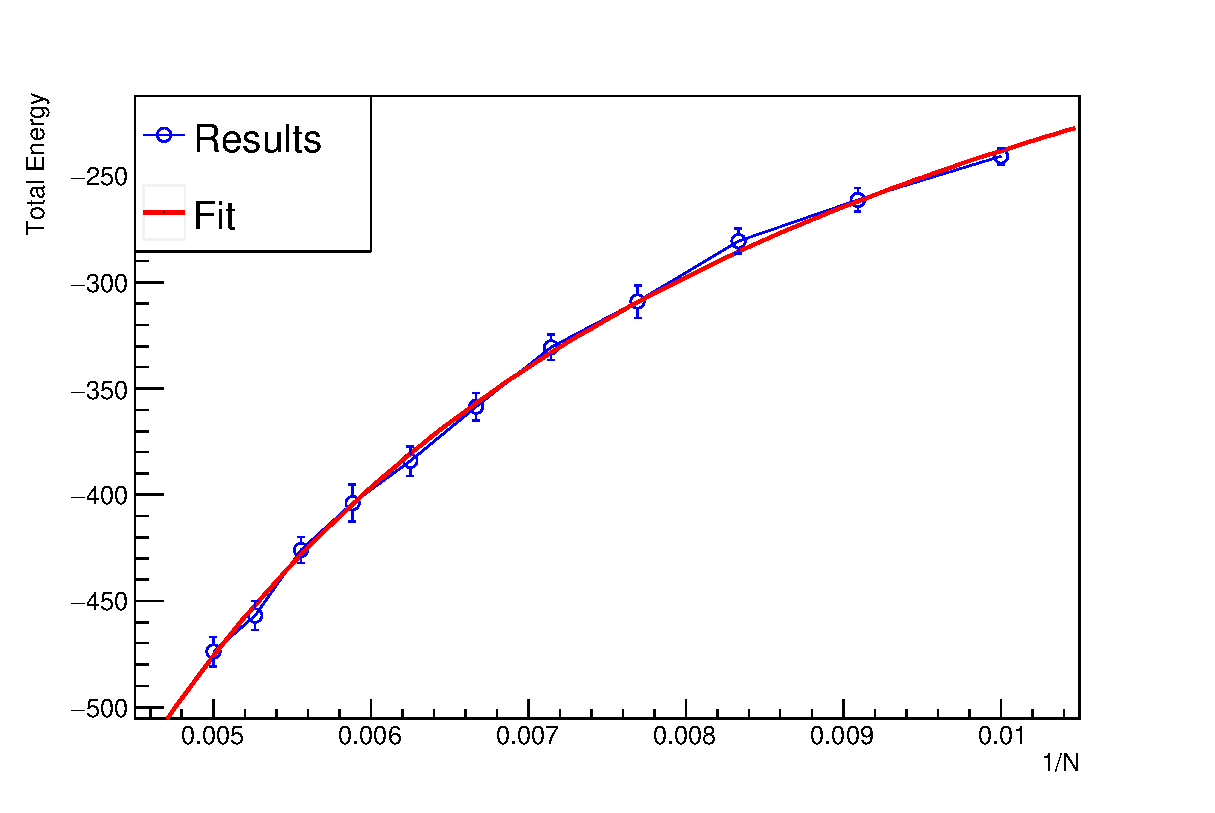
\includegraphics[height=0.2\textheight]{Root Fit/fit_exp1_p.eps}
		\caption{Average Energy}
	\end{minipage}\hspace{0.5cm}
	\begin{minipage}[t]{0.45\textwidth}
		\centering
		\includegraphics[height=0.2\textheight]{Root Fit/fit_exp1_flu.eps}
		\caption{fluctuations}
	\end{minipage}
\end{figure}
With periodic boundaries, we can seen that as $1/N\to 0$, $\ln \left| E_\text{tot} \right|$ raises linearly, so by going a fit with model $E = k\cdot \left(\frac{1}{N}\right)^{b}$ with CERN ROOT, 
by assigning energy's $1\sigma$ range with fluctuations, we can get:
\begin{equation}
	\left\{
		\begin{aligned}
			k &= \num[separate-uncertainty = true]{-2.38+-0.28}\\
			b &= \num[separate-uncertainty = true]{-9.99+-0.02}
		\end{aligned}
	\right.
\end{equation}
This result is somehow reasonable: energy per particle is a constant $\num[separate-uncertainty = true]{-2.38+-0.28}$ when $b = 1$. And when it comes to fluctuations, we can see $\delta U^2$ fit with same model 
\begin{equation}
	\left\{
		\begin{aligned}
			k &= 0.54\\
			b &= -1.00
		\end{aligned}
	\right.
\end{equation}
We can get $\delta U^2\propto N^{1.00}$ matches thermostatic result: $\delta U^2\propto N$.

\subsection{$T =0.728,\, \rho = 0.8442$, Hard Boundaries}
In this simulation, we get:
\begin{figure}[H]
	\centering
	\begin{minipage}[t]{0.45\textwidth}
		\centering
		\includegraphics[height=0.2\textheight]{Root Fit/fit_exp1_h.eps}
		\caption{Average Energy}
	\end{minipage}\hspace{0.5cm}
	\begin{minipage}[t]{0.45\textwidth}
		\centering
		\includegraphics[height=0.2\textheight]{Root Fit/fit_exp1_flu_h.eps}
		\caption{fluctuations}
	\end{minipage}
\end{figure}
With same fitting method, we can tell that for average energy
\begin{equation}
	\left\{
		\begin{aligned}
			k &= \num[separate-uncertainty = true]{-2.97+-0.91}\\
			b &= \num[separate-uncertainty = true]{-0.876+-0.06}
		\end{aligned}
	\right.
\end{equation}
This suggests that with hard boundaries, we can not easily do extrapolation, since $b$ is far away $1$.

And for fluctuation
\begin{equation}
	\left\{
		\begin{aligned}
			k &= 0.50\\
			b &= -1.02
		\end{aligned}
	\right.
\end{equation}
$\delta U^2\propto N^{1.02}$ approximately, $\delta U^2\propto N$

\subsection{$T =1.0,\, \rho = 0.1$, Periodic Boundaries}
In this simulation, we get:
\begin{figure}[H]
	\centering
	\begin{minipage}[t]{0.45\textwidth}
		\centering
		\includegraphics[height=0.2\textheight]{Root Fit/fit_exp2.eps}
		\caption{Average Energy}
	\end{minipage}\hspace{0.5cm}
	\begin{minipage}[t]{0.45\textwidth}
		\centering
		\includegraphics[height=0.2\textheight]{Root Fit/fit_exp2_f.eps}
		\caption{fluctuations}
	\end{minipage}
\end{figure}
\begin{equation}
	\left\{
		\begin{aligned}
			k &= \num[separate-uncertainty = true]{-0.275+-0.023}\\
			b &= \num[separate-uncertainty = true]{-1.02+-0.16}
		\end{aligned}
	\right.
\end{equation}
Because $b=1$ is within its range of the fit's $1\sigma$ range, we can extrapolation energy per particles to $N\to \infty$, $\num[separate-uncertainty = true]{-0.275+-0.023}$.

And for fluctuation
\begin{equation}
	\left\{
		\begin{aligned}
			k &= 0.11\\
			b &= -1.10
		\end{aligned}
	\right.
\end{equation}
Still, take error from the simulation info consideration, we can say that $\delta U^2\propto N$

\subsection{$T =1.0,\, \rho = 0.1$, Hard Boundaries}
In this simulation, we get:
\begin{figure}[H]
	\centering
	\begin{minipage}[t]{0.45\textwidth}
		\centering
		\includegraphics[height=0.2\textheight]{Root Fit/fit_exp2_h.eps}
		\caption{Average Energy}
	\end{minipage}\hspace{0.5cm}
	\begin{minipage}[t]{0.45\textwidth}
		\centering
		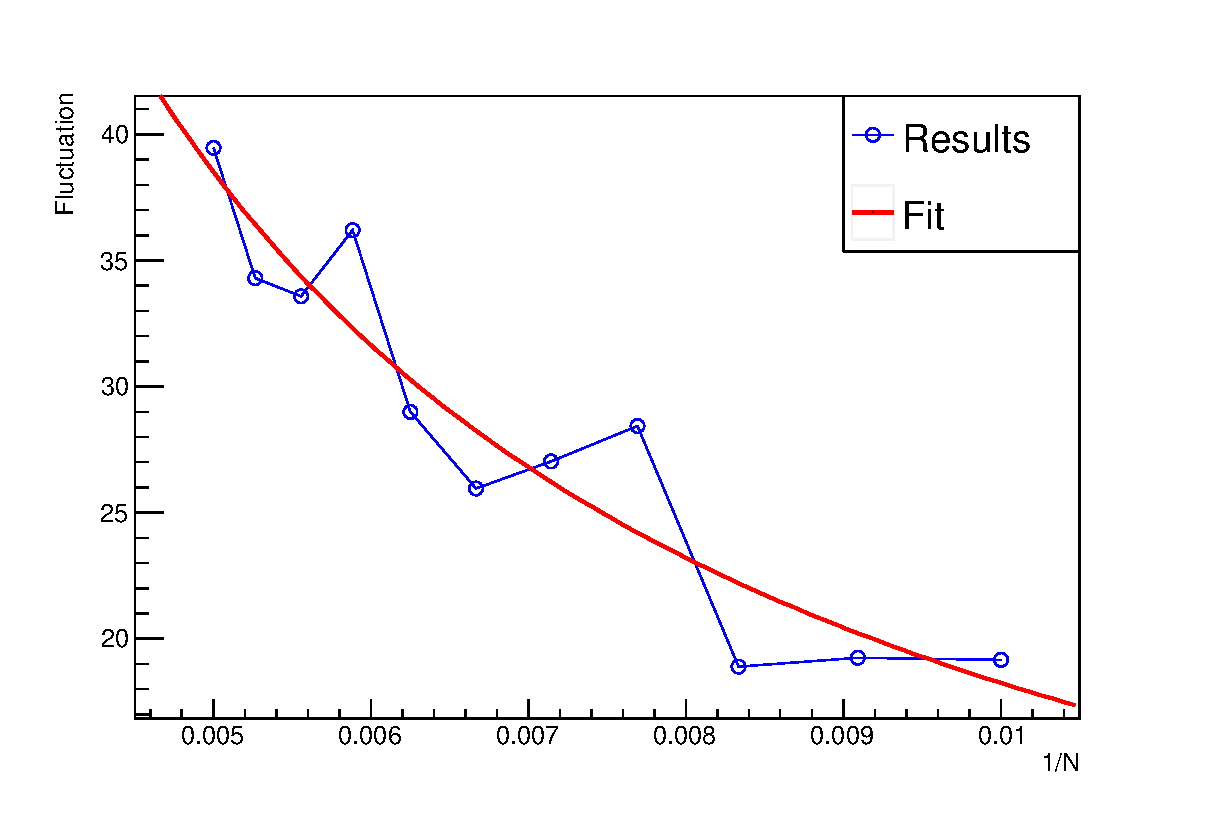
\includegraphics[height=0.2\textheight]{Root Fit/fit_exp2_f_h.eps}
		\caption{fluctuations}
	\end{minipage}
\end{figure}

\begin{equation}
	\left\{
		\begin{aligned}
			k &= \num[separate-uncertainty = true]{-0.285+-0.024}\\
			b &= \num[separate-uncertainty = true]{-1.00+-0.17}
		\end{aligned}
	\right.
\end{equation}
Because $b=1$ is within its range of the fit's $1\sigma$, we can extrapolation energy per particles to $N\to \infty$, $\num[separate-uncertainty = true]{-0.275+-0.023}$. 
Extrapolation works here for hard periodic boundaries suggest that for small density, difference between the two boundaries will be small enough.

And for fluctuation
\begin{equation}
	\left\{
		\begin{aligned}
			k &= 0.13\\
			b &= -1.07
		\end{aligned}
	\right.
\end{equation}
Still we can say, approximately, $\delta U^2\propto N$.

\section{Radial distribution function}
By simulation and save final particles positions, choose one and calculate its distance between other particles. Draw the result into a histogram. As following, 
all simulation is done with a random initialization:

\subsection{$T =0.728,\, \rho = 0.8442$}
\begin{figure}[h]
	\centering
	\includegraphics[height=0.2\textheight]{fig/exp1_rdf_peri_1.eps}
	\caption{histogram from simulation with $T =0.728,\, \rho = 0.8442,\, N=100$}
	\label{fig:rdf-1}
\end{figure}
Figure \ref{fig:rdf-1} is done with average histogram for all particles, and we can see a peak at near $x = 1.2$, and a wavy curve after. The change in density get smaller as 
r raises, finally stop on near average density.

By adding energy per bin, we can get particle energy from the histogram, it is $-2.360$. Slightly different from pervious simulation but within fluctuation range $U\pm\delta U$.

I guess, in this picture, the system is in liquid state, with medium coherence length.

\subsection{$T =1.0,\, \rho = 0.1$}
\begin{figure}[h]
	\centering
	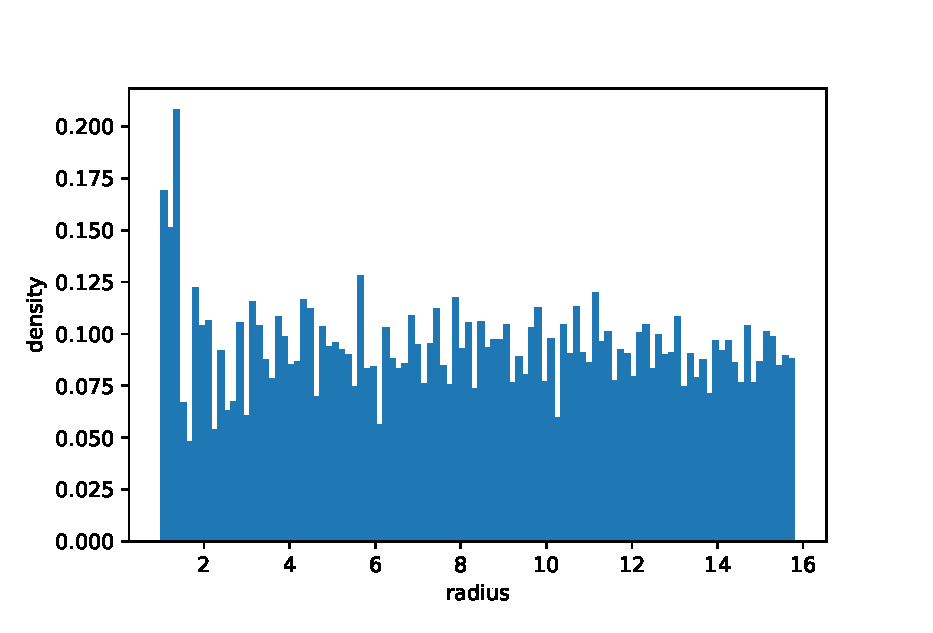
\includegraphics[height=0.2\textheight]{fig/exp2_rdf_peri_1.eps}
	\caption{histogram from simulation with $T =1.0,\, \rho = 0.1, \,  N = 100$}
	\label{fig:rdf-2}
\end{figure}
This time there is no such structure, here we can see that the radius distribution is likely uniform after one peak. Energy per particle is $-0.26$, still has a slightly difference but within 
fluctuation range $U\pm\delta U$, the two results matches.

This time, the system is in gas state, with small coherence length.
\subsection{$T =0.9,\, \rho = 1.1$}
\begin{figure}[h]
	\centering
	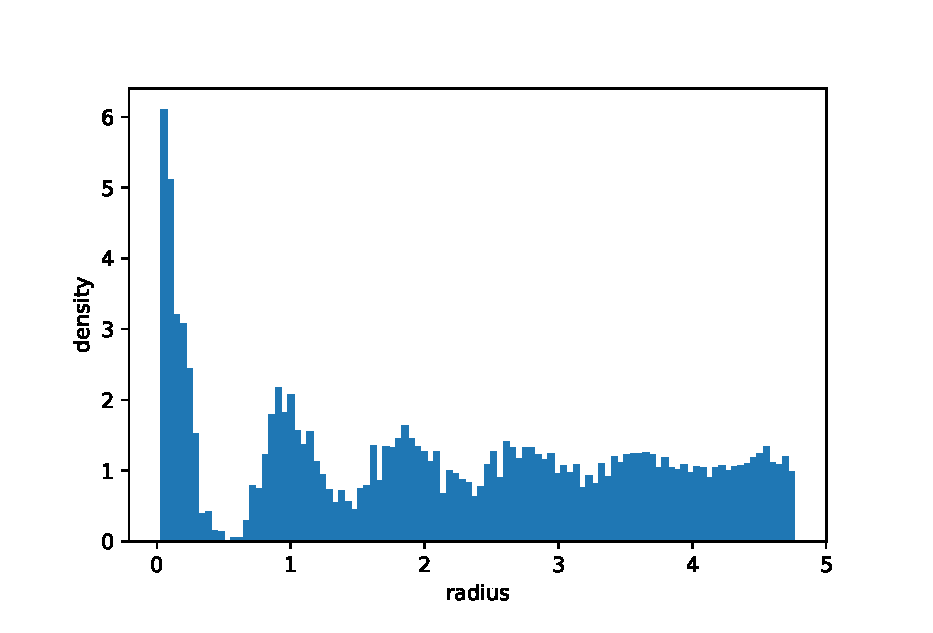
\includegraphics[height=0.2\textheight]{fig/rdf_exp3.eps}
	\caption{histogram from simulation with $T =0.9,\, \rho = 1.1, \,  N = 100$}
	\label{fig:rdf-3}
\end{figure}
With high density, we can see the approximate periodic structure in Figure \ref{fig:rdf-3}, this figure, clearly shows one peak after one, finally stop changing and stop at average density.

And energy per particle is $2.49$ from the histogram. Is is positive, which suggests that is very pressured. And the first peak is near to 6, is hexagonal's coordination number.

System is in solid state, with a high coherence length.
\section{Equation of state}
Use virial and pressure from the book:
\begin{equation}
	\left\{
		\begin{aligned}
			P&=\frac{\rho}{\beta}+\frac{\text{vir}}{V} \\
			\text{vir}&=\frac{1}{2} \sum_{i} \sum_{j>i} \mathbf{f}\left(\mathbf{r}_{i j}\right) \cdot \mathbf{r}_{i j}
		\end{aligned}
	\right.
\end{equation}
And the tail correction:
\begin{align}
	p_{\text{tail}} &= 
\end{align}

\end{document}